%!TEX root = paper.tex

We next moved on to develop a continuous erosion model that operates on smooth surfaces in contrast to our previous discrete one that operated on piecewise linear surfaces. Physically this new model represents a surface being worn down gradually, such as a bar of soap in water or an ice cube melting. 

\subsection*{Continuous Erosion Processes}

There are a wide range of different erosion processes, and most of them are far too complex for the scope of this paper. To generate simple simulations, we use key properties of the surface such as curvature and position as input variables to erosion functions.

We will start by introducing an explicit representation of a surface. This choice of using an explicit representation instead of an implicit one may seem odd to the reader, but we would like to stress that this was a conscious decision on our part because it paves the pay for the use of spectral methods to represent the surface, which we will discuss more in Section \ref{sec:numerical-modeling}. To represent the surface explicitly, we will introduce a parameter $s \in [0, 2\pi)$ that increases when moving counterclockwise around the surface. Now the surface can be represented by $\bvec{x}(s) = (x_1(s), x_2(s))$, for some functions $x_1(x), x_2(s)$. In contrast to modeling erosion as a discrete process, as was done in the previous section, we will now model it with the following differential equation

\begin{equation}
\label{eq:erosion-diff-eq}
\frac{d(\bvec{x}(s))}{dt} = g(s) \; \bhat{n}(s)
\end{equation}

for some function $g(\bvec{x}(s))$ that depends on the erosion process. $\bhat{n}(s)$ is the surface unit normal vector oriented inwards.

\subsection*{Example Surface}

The example shape that we will use for modeling our continuous processes is shown in Figure \ref{fig:blob-shape}.

\begin{figure}[H]
    \begin{center}
      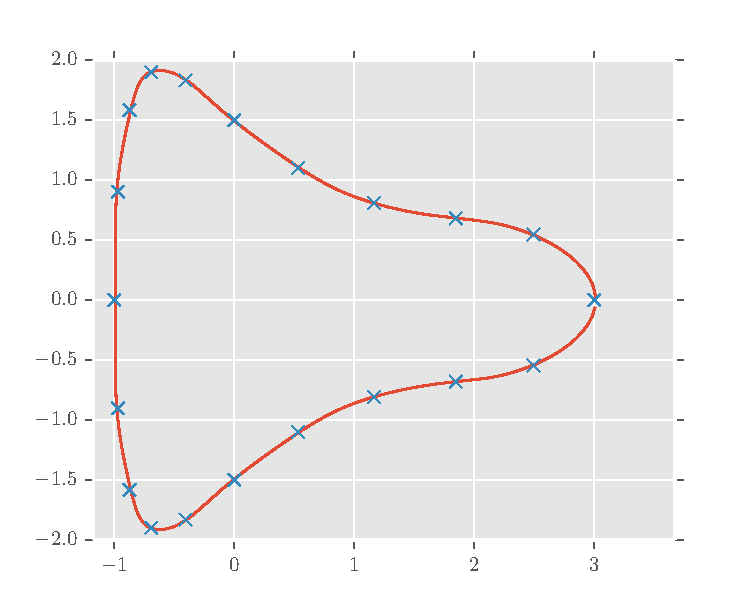
\includegraphics[keepaspectratio]{blob_shape.pdf}
    \end{center}
  \vspace{-.2in} % corrects bad spacing
  \caption{\label{fig:blob-shape} Example shape.}
\end{figure}

The equations for the shape are the following ($T_i$ is the i\textsuperscript{th} Chebyshev polynomial)

\begin{align*}
  x_1(s) = \cos(s) \paren{2 T_0\paren{\frac{s-\pi}{\pi}} + T_2\paren{\frac{s-\pi}{\pi}}}\\
  x_2(s) = \sin(s) \paren{2 T_0\paren{\frac{s-\pi}{\pi}} + T_4(\paren{\frac{s-\pi}{\pi}})}
\end{align*}

The method used to represent the shape numerically will be explained in Section \ref{sec:numerical-modeling}, but first we will take a moment to explain the various erosion processes that we will model in this section.

\subsubsection*{Smoothing Process}

One of the processes that we will look at is a soap bar being worn down by a person holding it in their hand, which we will call the \textit{Smoothing Process}. In this process, the corners of the surface will get worn down quickest, because they are the first parts of the surface to come into contact with the person's hand. Technically the furthest protruding bumps will be worn down quickest, but to simplify the problem, we consider every point of the surface to wear down at a rate proportional to the curvature at the point. We will use a signed curvature $\kappa$, so that a bump will have positive curvature, and an indentation will have negative curvature. $g(s)$ for this model is the following

\begin{equation}
g(\kappa(s)) = \tan^{-1}(\beta \, (\kappa(s) - \alpha)) + \frac{\pi}{2}
\end{equation}

For our simulations we chose $\alpha = 1, \; \beta = 5$ so that $g \le 3$ for the range of $\kappa$ along our trial surfaces ($\kappa \in [-2, 2]$). This restriction is not based on any physics of the problem, and was chosen purely for the aesthetic look of the resulting simulation.

\begin{figure}[H]
    \begin{center}
      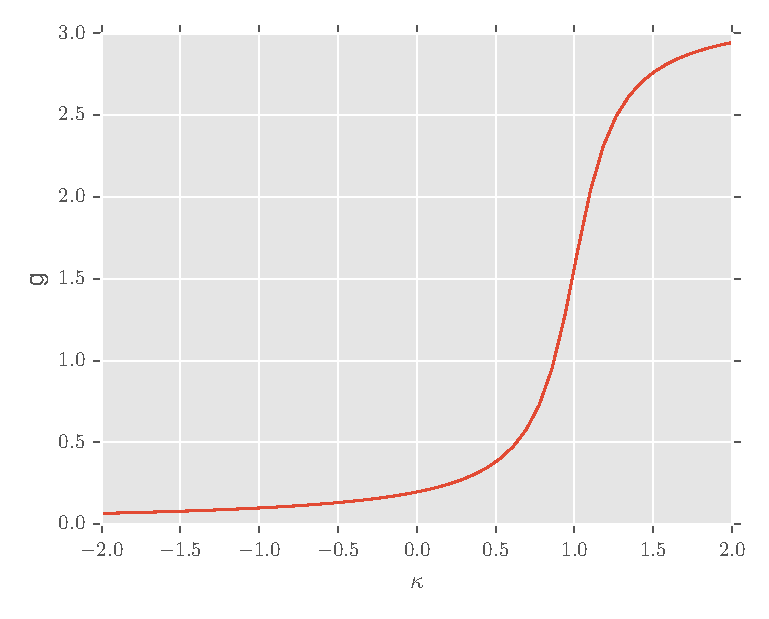
\includegraphics[keepaspectratio]{g_1.pdf}
    \end{center}
  \vspace{-.2in} % corrects bad spacing
  \caption{\label{fig:g-1} Plot of $g(\kappa)$ for \textit{Smoothing Process}.}
\end{figure}

\subsubsection*{Bottom Recession Process}

Our second process is an object sitting in a bath of acid, which we will call our \textit{Bottom Recession Process}. In this process, the lowest points (smallest values of $\bvec{x}_2$) on the surface will erode quickest. $g(\bvec{x})$ for this model is the following

\begin{align}
  f(\bvec{x})& = \frac{1}{\alpha \, (\bvec{x}_2 - x_{2, min}) + \beta} - \gamma\\
  g(\bvec{x})& = \begin{cases}
    f(\bvec{x}) \qquad &\text{for} \quad f(\bvec{x}) > 0\\
    0 \qquad &\text{otherwise}
  \end{cases}
\end{align}

For our simulations we chose $\alpha = 10, \; \beta = \gamma = 0.1$ so that $g \approx 1$ for $y \approx y_{min}$.

\begin{figure}[H]
    \begin{center}
      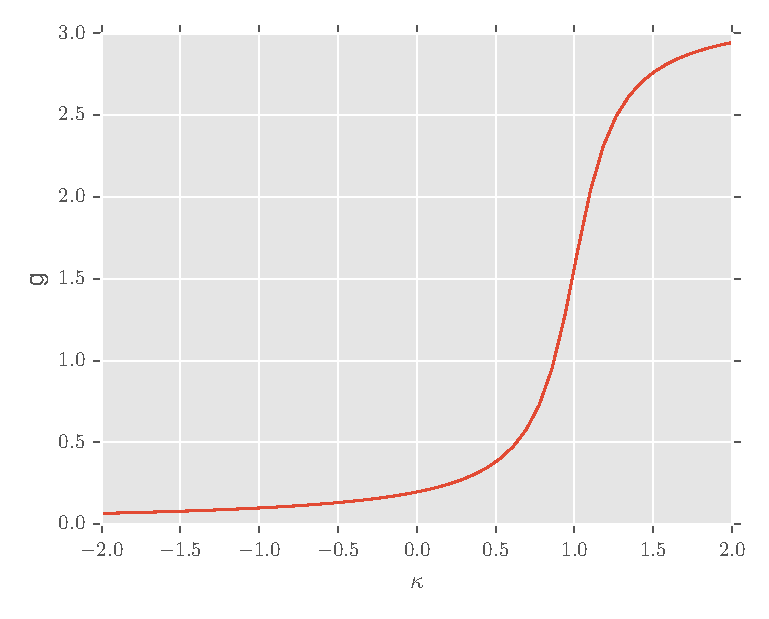
\includegraphics[keepaspectratio]{g_1.pdf}
    \end{center}
  \vspace{-.2in} % corrects bad spacing
  \caption{\label{fig:g-1} Plot of $g(\kappa)$ for \textit{Smoothing Process}.}
\end{figure}

\subsection*{Surface Equations}

To represent our surface numerically, we generate a matrix of evaluation points which are taken at locations $\bvec{s} = 2 \pi [0, 1/N, \dotsc, (N-1)/N]^T$ for some resolution $N$. This matrix $\bvec{x} \coloneqq \bracket{\bvec{x}_1(s), \bvec{x}_2(s)}$ is $N x 2$ and at each step in our simulation, we will evaluate the rhs of Equation \ref{eq:erosion-diff-eq} at the evaluation points.

To simplify our notation, we introduce the following vector calculus notation.

\begin{align*}
  \dot{\bvec{x}(s)}& \coloneqq \frac{d\bvec{x}}{ds}\\
  \ddot{\bvec{x}(s)}& \coloneqq \frac{d^2\bvec{x}}{dt^2}\\
  \kappa& = \frac{\dot{\bvec{x}} \times \ddot{\bvec{x}}}{\dot{x}^3} \tag{Curvature}
\end{align*}

\subsection*{Numerical Modeling}\label{sec:numerical-modeling}

We chose to model the surface parametrically with a Discrete Fourier series and use spectral methods for implementing Equation \ref{eq:erosion-diff-eq}. This is because spectral methods will maintain the smoothness of the surface much better than a local approximation of the surface using finite differences which only acts locally at points. When we refer to smoothness, we are really referring to how many derivatives of the function are bounded, or in other words, how quickly the Fourier coefficients go to $0$. Since, the surface is in $\R^2$, we will use the Real Fast Fourier Transform ($\mathcal{RFFT}$), since it is slightly faster than the standard Fast Fourier Transform (equations for the $\mathcal{RFFT}$ can be found in the appendix). 

To model the surface parametrically, we define a parameter vector $\bvec{s} = 2 \, \pi \, n / N, \qquad \text{for} \quad n = 0, \dotsc, N-1$. Now we let $\bvec{s}$ be a counterclockwise sampling of the surface at locations $\bvec{s}$ ($\bvec{s}$ can be scaled by a constant factor if the surface is not of length $2\pi$).

The $\mathcal{RFFT}$ allows us to calculate derivatives in $n \log{n}$ time. The following equations are derived in most introductory spectral method texts, so they will be stated without proof here

\begin{align}
  \dot{\bvec{x}}& = \mathcal{RFFT}^{-1}\paren{diag(i \, [0:N/2, 0]) \; \mathcal{RFFT}(\bvec{x})}\\
  \ddot{\bvec{x}}& = \mathcal{RFFT}^{-1}\paren{diag(i^2 [0:N/2+1]^2) \; \mathcal{RFFT}(\bvec{x})}
\end{align}

Note: $diag(\bvec{a})$ is the diagonal matrix with the elements of $\bvec{a}$ along the diagonal. Also, $\bvec{x}_1$ and $\bvec{x}_2$ are treated separately, e.g.\ $\mathcal{\mathcal{RFFT}}(\bvec{x}) \coloneqq [\mathcal{RFFT}(\bvec{x}_1), \mathcal{RFFT}(\bvec{x}_2)]$.

Using the above equations, the surface normal and surface curvature can now be quickly computed

\begin{align}
  \bhat{n}& = [-\dot{\bvec{x}}_2, \dot{\bvec{x}}_1]\\
  k& = \frac{\dot{\bvec{x}}_1 \ddot{\bvec{x}}_2 - \dot{\bvec{x}}_2 \ddot{\bvec{x}}_1}{\paren{\bvec{x}_1^2 + \bvec{x}_2^2}^{3/2}}
\end{align}

Forward time integration of Equation \ref{eq:erosion-diff-eq} can now be implemented with a standard ODE time stepping integration methods. In this paper, we used SciPy's {\tt odeint} method for integrating Equation \ref{eq:erosion-diff-eq}.

\subsection*{Point Collision Problems}

Unfortunately, the simplicity gained from modeling the surface with a Fourier series is soon lost when we start time stepping. As can be seen in Figure \ref{fig:remove-lowest-blob-bad}, the process works well for a short time period, but then the surface folds over itself (a physical impossibility).

\begin{figure}[H]
    \begin{center}
      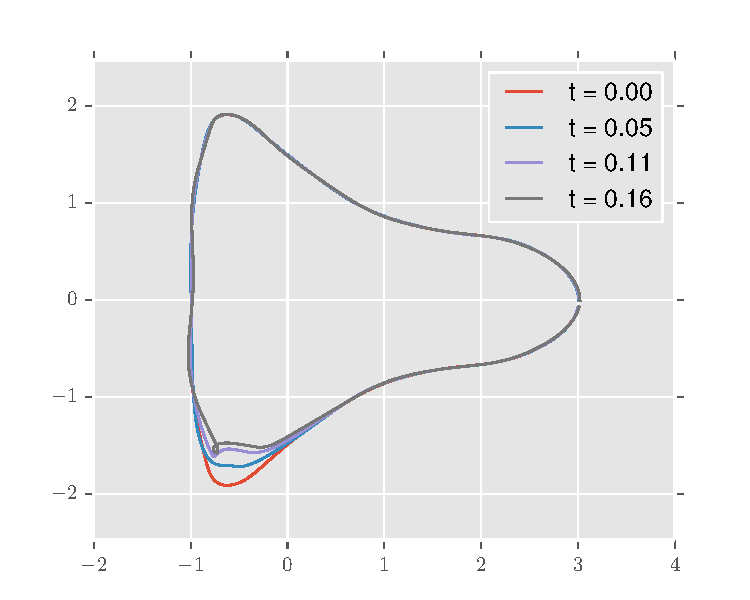
\includegraphics[keepaspectratio]{remove_lowest_blob_bad.pdf}
    \end{center}
  \vspace{-.2in} % corrects bad spacing
  \caption{\label{fig:remove-lowest-blob-bad}}
\end{figure}

To investigate why this occurs, we will show a zoomed in portion of the same figure, with the evaluation points shown. 

\begin{figure}[H]
    \begin{center}
      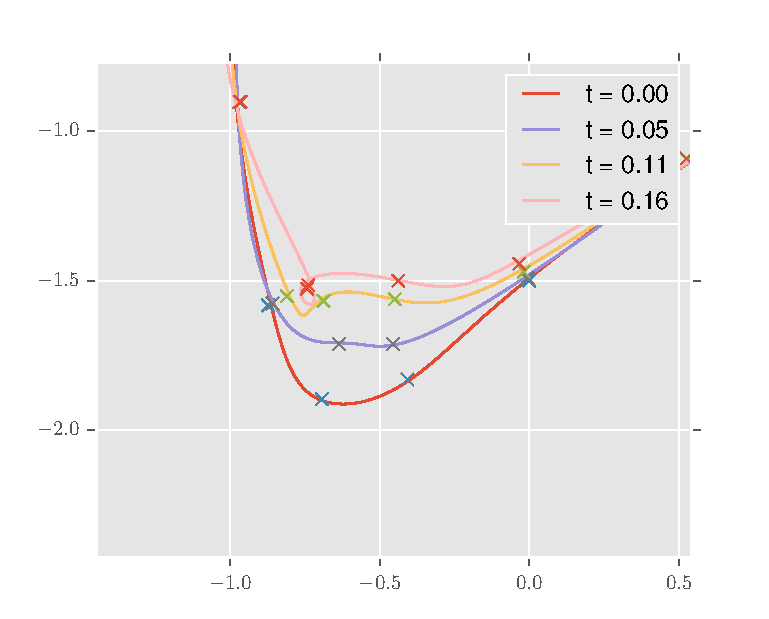
\includegraphics[keepaspectratio]{remove_lowest_blob_bad_zoom.pdf}
    \end{center}
  \vspace{-.2in} % corrects bad spacing
  \caption{\label{fig:remove-lowest-blog-bad-zoom}}
\end{figure}

Looking closely, it can be seen that areas of high curvature form when evaluation points get close to each other, and this eventually leads to surface folding. Our guess is that this occurs because we are using discrete time stepping, so there are errors in the approximation of the shape's change with time. This is fine when the evaluation points are far from each other, but when they get close to each other, the errors become significant and affect the direction of the surface unit normal vectors. The folding causes unit normal vectors of nearby points to point at each other and which subsequently causes the points to cross over each other.

\subsection*{Redistributing Points}

The most obvious way to fix this problem would be to redistribute the points evenly on the surface at every step. This wouldn't be too difficult of a task, since we can easily integrate and interpolate with the FFT and find a new set of evaluation points, $\bvec{x}$ that are evenly spaced on the surface. 

Unfortunately, if we arbitrarily move points around, we lose spectral accuracy, because our new points will be sampled at different parameter values $\tilde{s} \ne s$, but the Discrete Fourier transform assumes that the points are sampled at $s$. This parameter transformation is okay if there exists some smooth (ideally analytic) function, $h(s)$, such that $h(s) = \tilde{s}$. This technique of parameter transformation is utilized extensively in spectral methods involving Chebyshev polynomials which use $h(s) = \cos(s)$ to cluster evaluation points near both endpoints of the domain.

Redistributing points in such a way to ensure that $h(s)$ exists is difficult though, so we will first describe some different methods we attempted at eliminating the surface folding.

\subsection*{Continuous Redistribution}

To redistribute points, such that there exists some function $h(s)$ as described above we decided to model our redistribution by adding a term to Equation \ref{eq:erosion-diff-eq}, which is shown below. This works out nicely, because now the redistribution is smooth, so $h(s)$ must exist, as long as Equation \ref{eq:erosion-diff-eq-2} has a solution.

\begin{align}
  \label{eq:erosion-diff-eq-2}
  \frac{d\bvec{x}}{dt}& = g(x) \; \bhat{n} + \alpha \, \bvec{a}_t\\
  \bvec{a}_t& = \frac{\ddot{\bvec{x}} \cdot \dot{\bvec{x}}}{\norm{\dot{\bvec{x}}}} \; \frac{\dot{\bvec{x}}}{\norm{\dot{\bvec{x}}}}
\end{align}

Physically, $\bvec{a}_t$ is the component of $\ddot{\bvec{x}}$ tangent to the surface. The reasoning behind adding this term is that $\dot{\bvec{x}}$ is inversely proportional to the density of points on the surface; we want to shift points away from denser areas, which means moving them in the direction of larger $\dot{\bvec{x}}$ which is $\bvec{a}_t$. For the moment, we set $\alpha = 1$, since $\bvec{a}_t$ is of the same order as $g(x)$ for our surface. More analysis should be done in the future to best determine what $\alpha$ should be (it seems likely that the optimal would depend on $g(x)$). 

As can be seen in Figure \ref{fig:remove-points-blob-good}, this dramatically improves our algorithm.

\begin{figure}[H]
    \begin{center}
      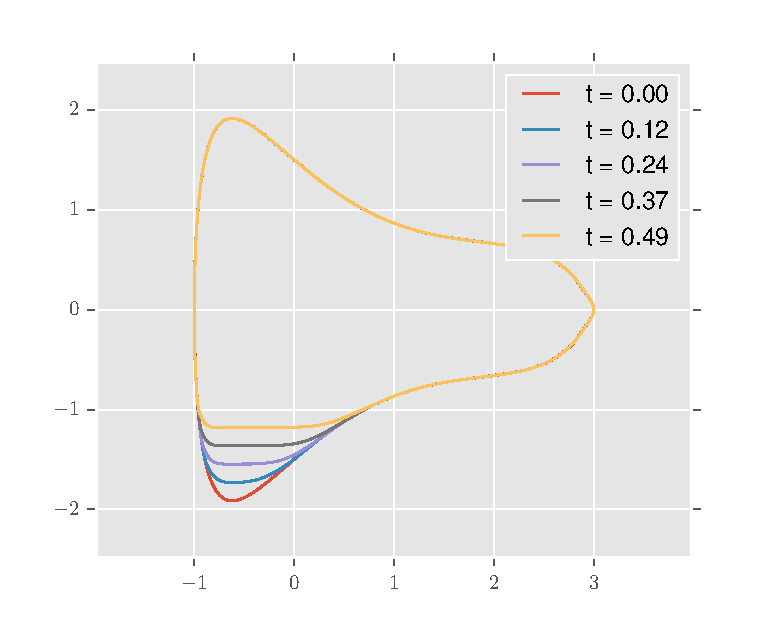
\includegraphics[keepaspectratio]{remove_points_blob_good.pdf}
    \end{center}
  \vspace{-.2in} % corrects bad spacing
  \caption{\label{fig:remove-points-blob-good}}
\end{figure}

If we plot the evaluation points (Figure \ref{fig:remove-points-blob-good-points}), it can be seen that the points redistribute themselves over time to stay evenly spaced on the surface.

\begin{figure}[H]
    \begin{center}
      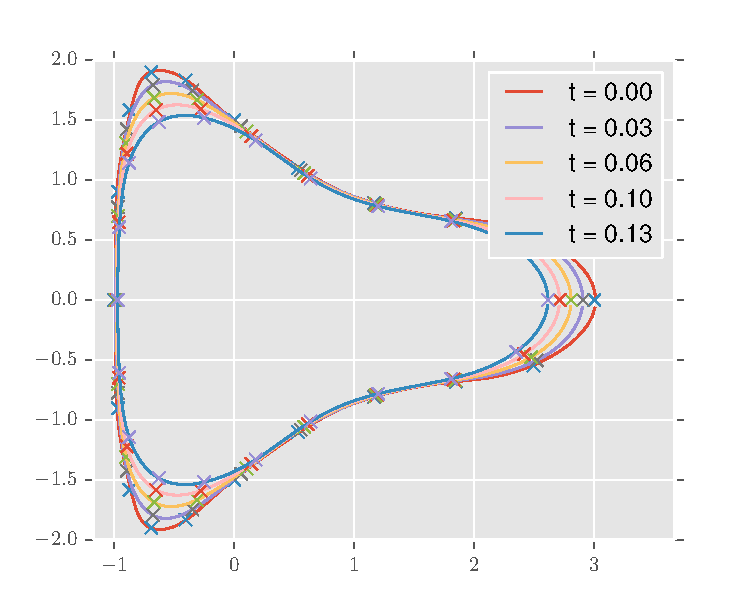
\includegraphics[keepaspectratio]{remove_points_blob_good_points.pdf}
    \end{center}
  \vspace{-.2in} % corrects bad spacing
  \caption{\label{fig:remove-points-blob-good-points}}
\end{figure}